\documentclass{article}
\usepackage[margin=1.25in]{geometry}
\usepackage{amsmath, amssymb, setspace, enumerate, enumitem}
\usepackage{setspace}
\usepackage{graphicx}
\onehalfspacing

\begin{document}
    \begin{enumerate}
        \item Exercise 1.3 in LFD
        \begin{enumerate}[label=(\alph*)]
            \item We can consider 2 cases for this problem, case 1 is that $x(t)$ is misclassified to $-1$ when it is supposed to be $+1$. In this case, $y(t)$ should equal $+1$, and $x(t)$ should equal $-1$, the product of any number with a negative number is always negative. The other case would be $x(t) = +1$, and $y(t) = -1$, where the same rule will apply.
            \item begin with the left hand side of the inequality
            \begin{align*}
                y(t)w^T(t+1)x(t) &= y(t)(w^T(t) + y(t)x(t))x(t)\\
                &= y(t)w^T(t)x(t) + y(t)^2x(t)^2\\
                y(t)w^T(t)x(t) + y(t)^2x(t)^2 & > y(t)w^T(t)x(t)
            \end{align*}
            Since $y(t)^2x(t)^2$ is always positive, the inequality will always hold.
            \item For any $x(t)$, it is correctly classified if $y(t)w^T(t)x(t) > 0$. In part (b), we proved that $y(t)w^T(t+1)x(t) > y(t)w^T(t)x(t)$, so if $y(t)w^T(t)x(t) > 0$, then $y(t)w^T(t+1)x(t) > y(t)w^T(t)x(t)$, meaning the update rule is always moving towards a larger number, for any amount $x(t)$ that is misclassified, it will continue to increase until $y(t)w^T(t)x(t) > 0$. 
        \end{enumerate}

        \item Exercise 1.5 in LFD
        \begin{enumerate}[label=(\alph*)]
            \item Learning: use data to see how people of different ages react to the medical test
            \item Design: a simple calculation suffices
            \item Learning: many types of fraud possibilities
            \item Design: a simple calculation suffices
            \item Learning: use data to determine how traffic is with different traffic light timings
        \end{enumerate}

        \item Exercise 1.6 in LFD
        \begin{enumerate}[label=(\alph*)]
            \item Supervised: training data are the books that they previously liked.
            \item Supervised \& Reinforcement: supervised training data will be past tic tac toe games, reinforcement learning will be putting a higher grade for the games won and a lower grade for the games lost, and each following game, it will look at the data with higher grade.
            \item Unsupervised: Clusters of movies with more or less the same genre
            \item Reinforcement \& Unsupervised: Reinforcement learning will give a grade to how well the music sounds, if it sounds good, keep playing like that. Unsupervised learning will be to listen to music that sounds similar to the music that sounds good.
            \item Supervised: Use data of people who paid off their debt and people who have defaulted
        \end{enumerate}

        \item Exercise 1.7 in LFD
        \begin{enumerate}[label=(\alph*)]
            \item 3: $f8$ \\ 2: $f4, 6, 7$ \\ 1: $f2, 3, 5$ \\ 0: $f1$
            \item 3: $f1$ \\ 2: $f2,3,5$ \\ 1: $f4,6,7$ \\ 0: $f8$
            \item 3: $f2$ \\ 2: $f1, 4, 6$ \\ 1: $f3,5,8$ \\ 0: $f7$
            \item 3: $f7$ \\ 2: $f3,5,8$ \\ 1: $f1,4,6$ \\ 0: $f2$
        \end{enumerate}

        \item Problem 1.1 in LFD
        \begin{verbatim}
            P[A: 2nd black | B: 1st black] = P[both black] / P[1st black]
            P[both black] = 1/2 -> has to land in the black bag
            P[1st black] = 3/4 -> excludes when white ball is chosen
            P[A: 2nd black | B: 1st black] = (1/2) / (3/4) = 2/3
        \end{verbatim}

        \item Problem 1.2 in LFD
        \begin{enumerate}[label=(\alph*)]
            \item The line that separates $h(x) = +1$ and $h(x) = -1$ is $w_0 + x_1w_1 + x_2w_2 = 0$, which we could rearrange to
            \begin{align*}
                x_2 &= -\frac{x_1w_1}{w_2} - \frac{w_0}{w_2}\\
                &= -\frac{w_1}{w_2}x_1 - \frac{w_0}{w_2}
            \end{align*}
            Here, $a = -\frac{w_1}{w_2}$ and $b = -\frac{w_0}{w_2}$

            \item For $w = [1,2,3]^T$, $a = -\frac{2}{3}$ and $b = -\frac{1}{3}$. For $w = -[1,2,3]^T$ $a = -\frac{-2}{-3}$, and $b = -\frac{-1}{-3}$. Since $a$ and $b$ are the same, the lines are the same.
            \begin{center}
                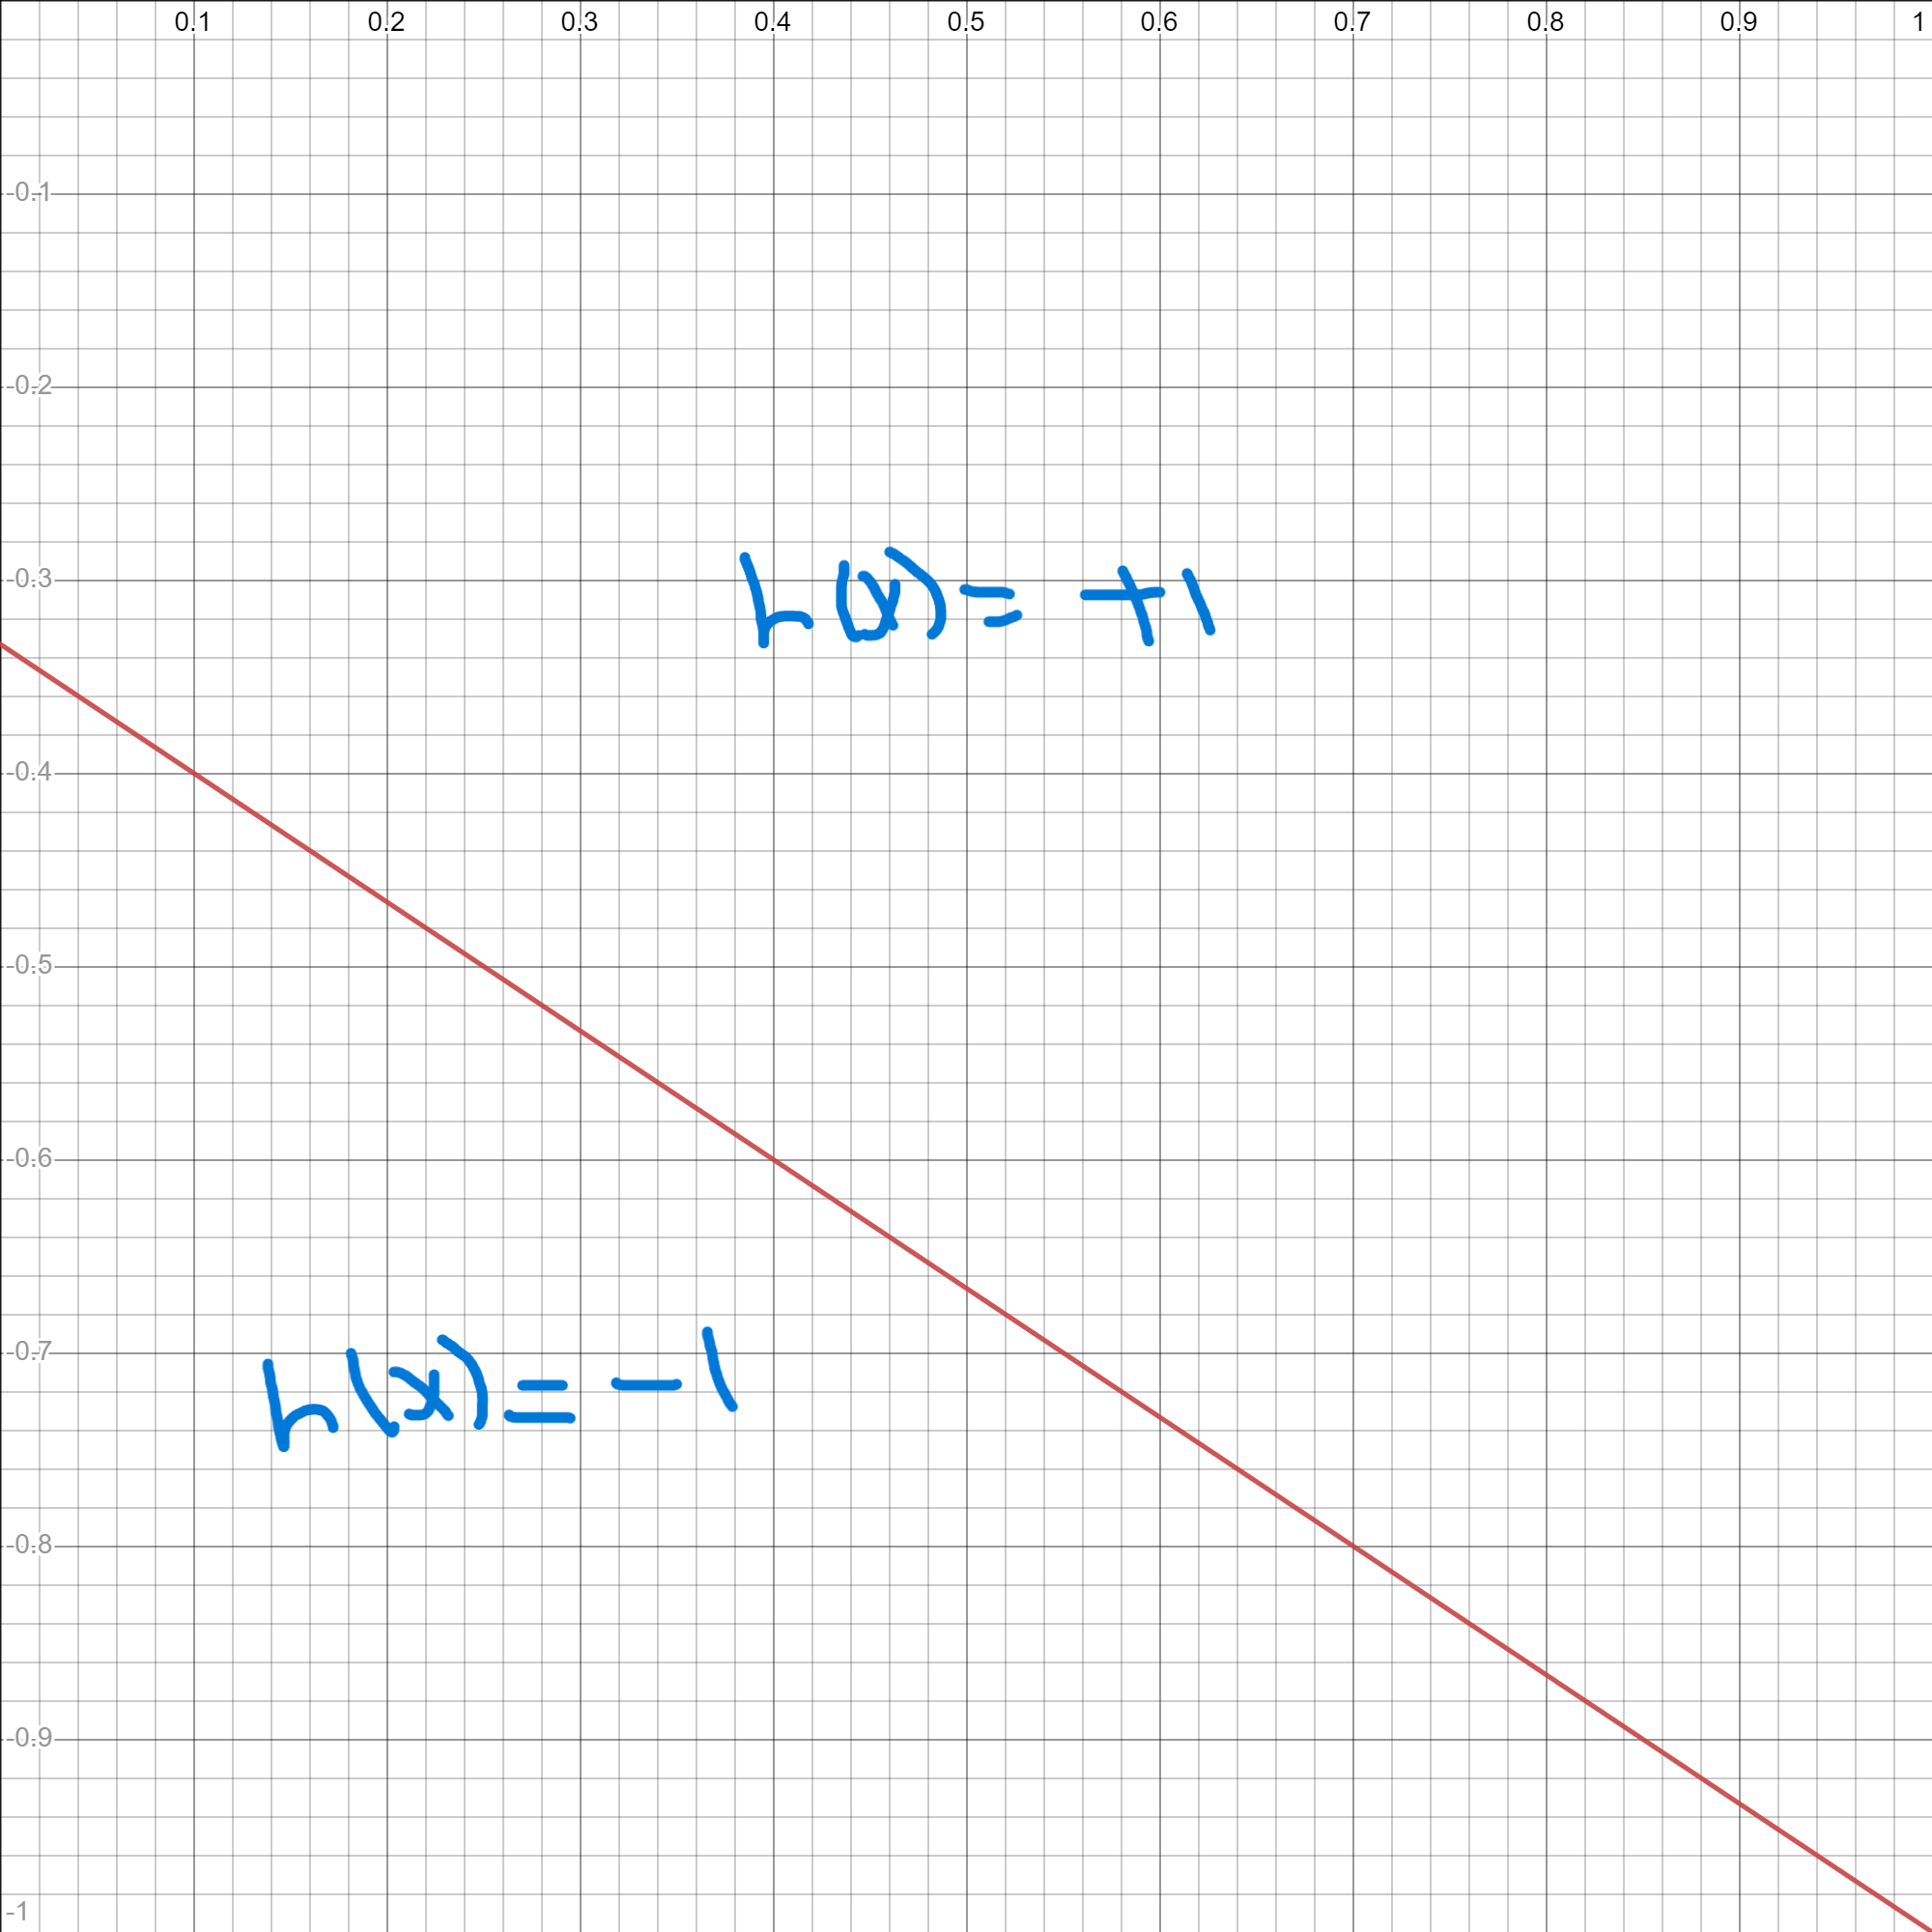
\includegraphics[scale=0.20]{images/desmos-graph.png}
            \end{center}
        \end{enumerate}

        \item Problem 1.4 in LFD
        \begin{enumerate}
            \item target function and randomly generated points \\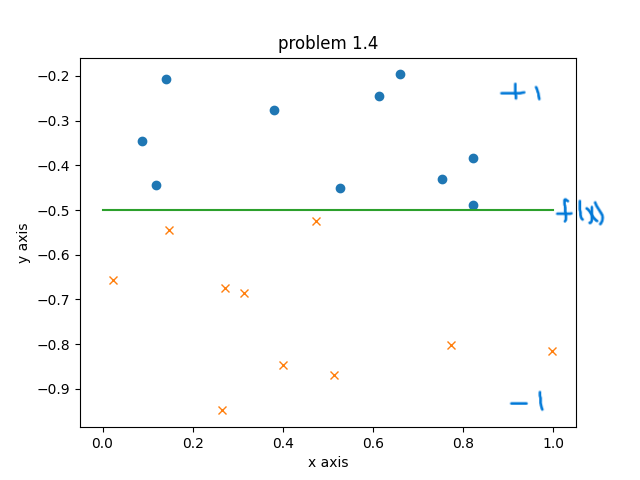
\includegraphics[scale=0.5]{images/a.png}
            \item 33 updates: target(f) is close to hypothesis(g), but there can still be improvement \\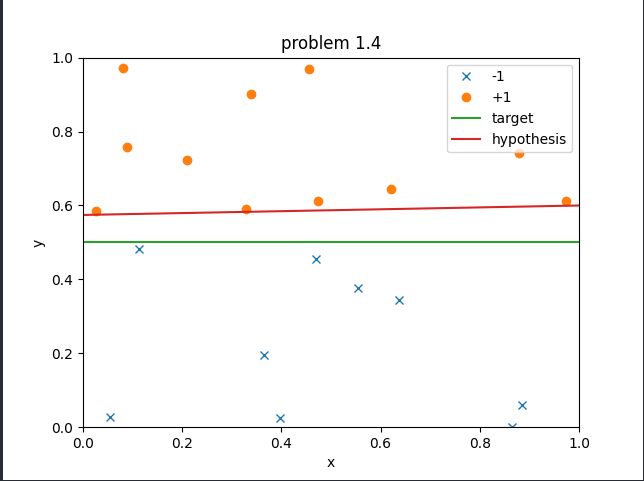
\includegraphics[scale=0.5]{images/b.png}
            \item 16 updates: plot is similar to (b), less updates but with so little data, it is an undeterminate difference \\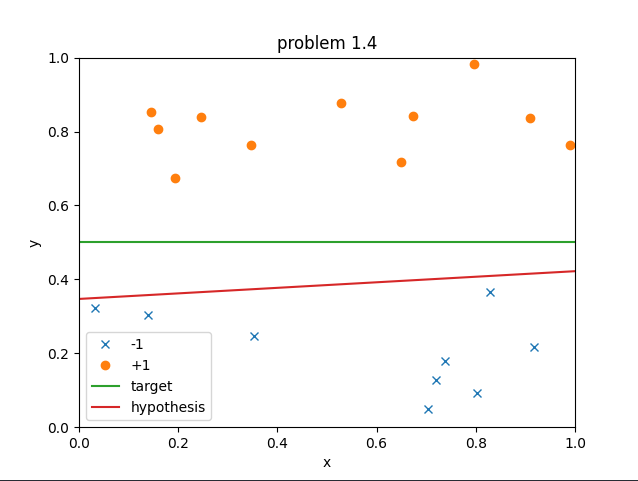
\includegraphics[scale=0.5]{images/c.png}
            \item 1496 updates: hypothesis(g) is a lot closer to target(f) compared to (b), a substantial increase in the number of iterations \\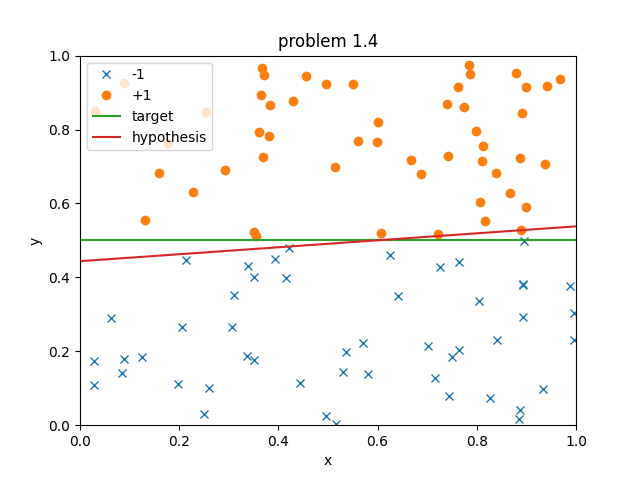
\includegraphics[scale=0.5]{images/d.png}
            \item 1212 updates: hypothesis(g) is basically the same line as target(f), more updates compared to (b) \\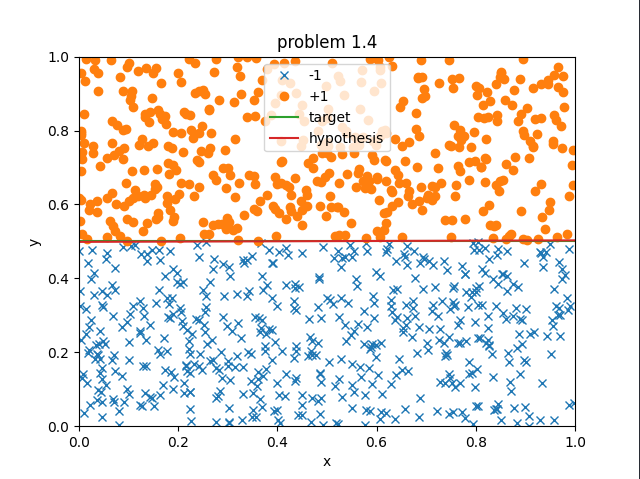
\includegraphics[scale=0.5]{images/e.png}
        \end{enumerate}
    \end{enumerate}
\end{document}